%%%%%%%%%%%%%%%%%%%%%%%%%%%%%%%%%%%%%%%%%
% Simple Sectioned Essay Template
% LaTeX Template
%
% This template has been downloaded from:
% http://www.latextemplates.com
%
% Note:
% The \lipsum[#] commands throughout this template generate dummy text
% to fill the template out. These commands should all be removed when 
% writing essay content.
%
%%%%%%%%%%%%%%%%%%%%%%%%%%%%%%%%%%%%%%%%%

%----------------------------------------------------------------------------------------
%	PACKAGES AND OTHER DOCUMENT CONFIGURATIONS
%----------------------------------------------------------------------------------------

\documentclass[12pt]{article} % Default font size is 12pt, it can be changed here

\usepackage{geometry} % Required to change the page size to A4
\geometry{a4paper} % Set the page size to be A4 as opposed to the default US Letter

\usepackage{graphicx} % Required for including pictures

\usepackage{float} % Allows putting an [H] in \begin{figure} to specify the exact location of the figure
\usepackage{subcaption}
\usepackage{mwe}
\usepackage{wrapfig} % Allows in-line images such as the example fish picture

\usepackage{lipsum} % Used for inserting dummy 'Lorem ipsum' text into the template
\usepackage{biblatex}
\usepackage{mathtools}
\linespread{1.2} % Line spacing

%\setlength\parindent{0pt} % Uncomment to remove all indentation from paragraphs

\graphicspath{{Pictures/}} % Specifies the directory where pictures are stored

\begin{document}

\section{Introduction}

Overhead Persistent InfraRed (OPIR) sensors are used in satellites to find interesting heat signatures. To better understand how filters will apply to data, test new filters, and testing applications we designed a simulation of OPIR data.

\section{Simulation}

The simulation of this data is intended to be as close to the real data as possible. In an attempt to achieve this, we must consider three important pieces of information: background noise, signal, and detector limits.

\subsection{Background Noise}\label{sec:Background}

Thermal noise is easily modeled by a Rayleigh Distribution. Rayleigh Distributions are characterized by a large peak at a given value with a lingering tail to higher values, see figure \ref{fig:Rayleigh_Dist}. The probability distribution function (PDF) of a Rayleigh Distribution  is 

\begin{figure}[h]
\centering
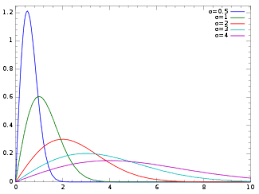
\includegraphics[width=\textwidth]{Rayleigh.png} 
\caption{Example of Rayleigh Distribution from Wikipedia. Notice the only difference in distributions is due to the change in $\sigma$.}
\end{figure}


\begin{equation}
f(x;\sigma) = \frac{x}{\sigma^2} e^{-\frac{x^2}{2 \sigma^2}}
\end{equation}

where x is the variable (greater than or equal to zero), and $\sigma$ is the scale parameter. Setting $\sigma$ is very simple, as the mean of the distribution is

\begin{equation}
\bar{x} = \sigma \sqrt{\frac{\pi}{2}}
\end{equation}

By choosing a value for the mean of your distribution, you can find the $\sigma$ for the distribution. 

To use this distribution, we must calculate the Cumulative Distribution Function (CDF), which is merely the integral of the PDF.  The CDF is normalized to 1 over the domain of [0,$\infty$), as this means there is a 100$\%$ of getting a value. 

\begin{equation}
F(x,\sigma) = \int_{0}^{x}   \frac{x}{\sigma^2} e^{-\frac{x^2}{2 \sigma^2}}dx = 1-e^{-\frac{x^2}{2 \sigma^2}}
\end{equation}

We use this CDF to find a value for the thermal noise in this manner. We invert the CDF, solving for the value of x:

\begin{align*}
F(x,\sigma) = y &= 1-e^{-\frac{x^2}{2 \sigma^2}} \\
e^{-\frac{x^2}{2 \sigma^2}} &= 1-y \\
\frac{x^2}{2 \sigma^2} &= - \ln \left(1-y\right) \\
x &= \sqrt{-2 \sigma^2 \ln \left(1-y\right)}\\
\end{align*}

By choosing a random number between 0 and 1 for y, we now get a value of our thermal noise (x). This distribution follows the Rayleigh Distribution and is easily change to different variations due to the $\sigma$ dependence.

\subsection{Signal}

The signal strength is the most straight forward component. A 'signal' is defined as a signature that does not deviate in strength. For simulation purposes, that signal strength can be drawn from a flat distribution. There are minor modifications to the signal to help simulate realistic conditions. The signal could move around the image, it could start at a low signal strength and gain in power, or start strong and weaken in strength. 

\subsection{Detector limits}

Every detector has unique capabilities and limits: resolution, field of view, saturation, frequency of capture to name a few. Those need to be handled with care in a simulation to make sure the concepts being tested work with that detector. These limitations work on a case by case basis, but the few encountered in simulation are the frequency of capture and the saturation of the cameras. Frequency of capture informs us how often the detector saves information. Saturation tells us the strongest signal the detector can save. For example, a detector may have a saturation of 50W. Signal one has a strength of 51W and signal two has a strength of 75 W. the detector would read both of those signals as having a strength of 50W due to saturation. You cannot make the saturation arbitrarily high, as there are other limits that need to be balanced against the saturation.

\section{Implementation}

The currently implementation of the simulation is written in python. The program asks for some items when starting up:

\begin{enumerate}
\item{Size of X-dimension of array (pixels)}
\item {Size of Y-dimension of array (pixels)}
\item{Frequency of Capture (Hz), f}
\item{Length of record (sec), t}
\item{Include background noise}
\item{Fine noise or coarse [COARSE NOT FULLY IMPLEMENTED]}
\item{Filtering Algorithm}
\end{enumerate}

After that has been set, the algorithm will run according to those presets. The algorithm will calculate how many snapshots it must make, freq*time. It will choose a random number of signal events and a random time between (0,t) for each signal to appear in the image. 

The procedure for the image is also very simple. For every pixel in the image, we get a thermal noise using the algorithm described in section \ref{sec:Background}. For that same pixel, we ask if a signal event is occupying that pixel at that time. If yes, we add the signal strength to that pixel. If no, we move on to the next pixel in the array. If the pixel value is above a saturation limit, we force the limit onto that pixel. 

This method is done for every pixel in the array, for every snapshot of simulation. This can be quite time consuming depending on the size of the array and there may be a way to speed up the calculations to reduce time. 

If a filter is applied, before saving the information the pixel value is run through the filter.  The 2 working filters are First Order Filter and Weightd Average Filter. The first order filter uses a simple equation to help filter the image

\begin{equation}
\rm{P[i,j,t]} = \rm{decay*X[i,j,t]} - (1-\rm{decay})*P[i,j,t-1]
\end{equation}

where P is the output value for the filtered pixel, decay is a constant, and X is the non-filtered pixel value at that time, and P[i,j,t-	1]] is the pixel value from the previous time frame. This filter has been used in other programs, and is easily adjustable by changing the value of the decay constant. The difference between filtered and non-filtered can be seen in figure \ref{fig:FO}.

\begin{figure}[h]
\begin{subfigure}[t]{.5\textwidth}
\centering

\includegraphics[width=\textwidth]{Sim.png} 
\caption{Non-filtered Simulation example.}
\end{subfigure}
\begin{subfigure}[t]{.5\textwidth}
\centering
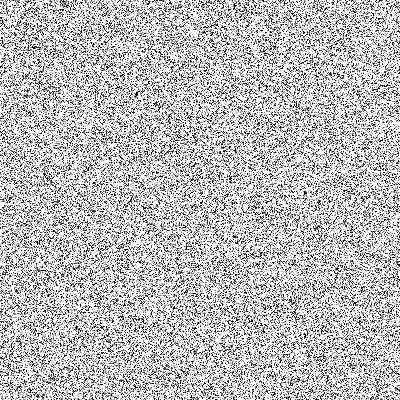
\includegraphics[width=\textwidth]{FO.png} 
\caption{First Order Filter Applied to Simulation.}
\end{subfigure}
\caption{An example of the first order filter at work. The left image is the simulation without the filter, while the right figure has the First Order Filter applied}
\label{fig:FO}
\end{figure}



The Weighted Average filter is seeking to take advantage of the fluctuations in the thermal noise. When averaging, signal has a constant strength, so the average will be approximately the same as the signal strength. But thermal noise fluctuations will vary wildly either up or down. By averaging the noise, we can attempt to suppress it to a lower value. We average over 3 samples from the past: $\rm{t_0,t_0 -1, t_0-2}$. We give weights to each value, with the current time having the largest weight and the latest time having the smallest. The equation for this filter is

\begin{equation}
\rm{P[i,j,t]} = \sum_{k=0}^{2} \rm{Weight[k]*X[i,j,t-k]}
\end{equation}

where P[i] is the filtered value of the pixel, X[i-k] is the read in value at that pixel, and Weight[k] is the weight given to that pixel. The difference between filtered and non-filtered can be seen in figure \ref{fig:WeightedAvg}

\begin{figure}[h]
\begin{subfigure}[t]{.5\textwidth}
\centering

\includegraphics[width=\textwidth]{Sim.png} 
\caption{Non-filtered Simulation example.}
\end{subfigure}
\begin{subfigure}[t]{.5\textwidth}
\centering
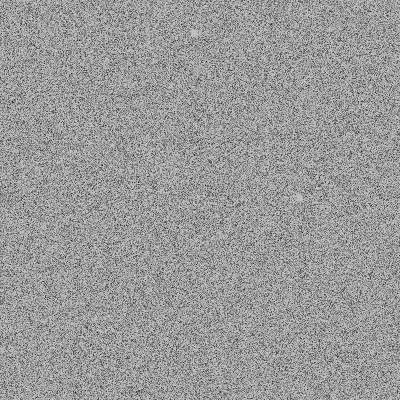
\includegraphics[width=\textwidth]{WA.png} 
\caption{Weighted Average Filter Applied to Simulation.}
\end{subfigure}
\caption{An example of the weighted average filter at work. The left image is the simulation without the filter, while the right figure has the Weight Average Filter applied}
\label{fig:WeightedAvg}
\end{figure}










\end{document}